%\section{Perceptron}
\label{sec:application:feedforward}

This section outlines how we have applied static feedfoward networks to our time series. For this purpose we used the MatLab toolbox for neural networks.

As a first attempt, we evaluated the Perceptron shown in \figref{perceptronbuildt}. 
It consists on a neuron with:
a number of set of inputs equals to the amount of physiologycal signals,
the hyperbolic tangent sigmoid as activation function
and $\text{bias}=0$. The training algorithm is, of course, the backpropagation.
\begin{figure}[!ht]
\centering
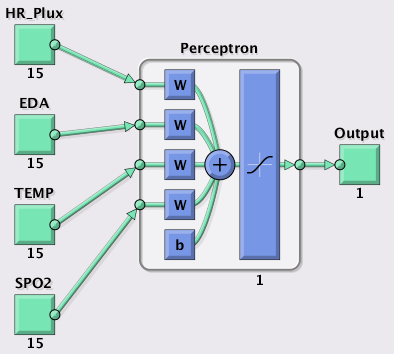
\includegraphics[width=0.5\columnwidth]{images/results/perceptronnn}
\caption{Perceptron neuron evaluated}
\label{fig:perceptronbuildt}
\end{figure}

As Perceptrons are static (\ie, without memory), each time series is truncated in every step with a window length of 15 samples. 
With the set of samples formed by the all the signals (a total of $4*15=60$ input samples), an unique output sample is computed. Notice that all the samples of the entire time-window is introduce at once, losing the temporal characteristic of the time series. During the implementation process, we set the length of the window to the range $\in [10,50]$. The larger the window is, more computation capacities are needed.

The configuration term that lasts is the forecasting horizon. We denote it as $n_{k}$ and it expresses the number of future time steps the algorithm is able to anticipate.
In the feedforward networks implemented, the prediction horizon is set by advancing in time the output. 
Hence, with $n_{k}=3$ for example, the samples of the windowed signals aligned in $t=t_{0}$ are forced to produce the output sample of $t=t_{3}$.
During our experiment, we set $n_{k}\in [10,50]$. 

As we could imagine, the results differ hugely from the desired behaviour of the network: we can see in the example depicted in \figref{perceptronResults}) how the Perceptron output is not capable of ``following'' the target signal.
Also reducing the set of physiological signals used as inputs or changing the length of their time-window, we obtained the similar ones.
\begin{figure}[!ht]
\centering
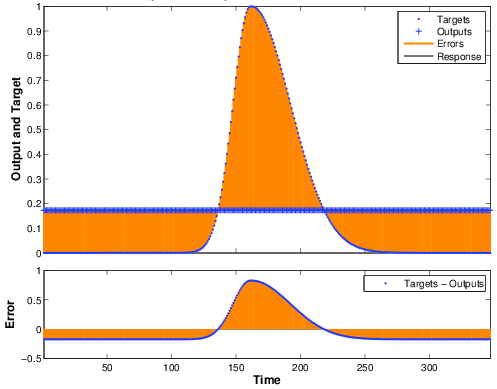
\includegraphics[width=0.7\columnwidth]{images/results/perceptronResults}
\caption{Example of the Perceptron neuron results}
\label{fig:perceptronResults}
\end{figure}



%We also experiment with a multilayer perceptron as the one shown in \figref{}. We performed simultations windowing the signals the same way (same window length) and with a semi-randow window. The latter case is the one that \figref{} depicts.



